% Chapter 模块对象设计

\subsection{模块对象设计}
由于使用的是基于ECMAScript262的NodeJS为基本开发语言,因此并没有传统面向对象中的类,但并不能说其不支持面向对象的特性。我基于Express.js开发了一个数据库连接工具——express-model,另外它也是一个建模工具,系统中所有的模型都被放在根目录下一个叫models的文件夹中,下面分别对其中的文件进行描述。

\subsubsection{express-model}
在描述对象模型之前,先来看看如何使用express-model,首先是更加仔细地对它进行一段描述:它为Express框架提供Model支持,可集成多种数据库(SQL \& NoSQL),灵活性高的轻量级工具。 由于Express官方并未显式地提供Model支持,express-model不仅能有效嵌入Express Mvc中,还支持多种需要Model的场景。模型作为MongoDB与Express的接口,实现了两端数据的同步功能。
\par

\noindent
\texttt{\large 创建一个Model:}

% create a model in express-model

\lstset{language=C}

\begin{lstlisting}[frame=single]
Models.define('yourModelName', function(exports) {
	exports.name = 'express-model 1.0'
	exports.getName = function() {
		return this.name
	}
})
\end{lstlisting}

\noindent
\texttt{\large 使用Model:}

% use a model in express-model

\lstset{language=C}

\begin{lstlisting}[frame=single]
var model = Models.use('yourModelName', function() {
	this.someVariable_1 = 1;
	this.someVariable_2 = 2;
})
response.render('yourViewName', model)
\end{lstlisting}

\subsubsection{user.js}

\noindent
\texttt{\large 其模型定义代码如下:}

% use a model in express-model

\lstset{language=C}

\begin{lstlisting}[frame=single]
var UserSchema = new Db.Schema({
	name: String,
	email: String,
	password: String,
	role: String
})
UserSchema.index({ name: 1, role: 1 })
\end{lstlisting}

\noindent
user.js模型主要用于管理用户与组相关的操作。它提供了一些方法供http服务端请求调用:

\begin{description}
	\item[toJSON] 将users对象重新组合,转换为更适合前端请求的json形式;
	\item[add] 用于注册新用户时,将请求的新用户数据同步到数据库服务器中;
	\item[view\_homepage] 用于视图页homepage,为其提取相关的信息;
\end{description}

\subsubsection{groups.js}

\noindent
\texttt{\large 其模型定义代码如下:}

% use a model in express-model

\lstset{language=C}

\begin{lstlisting}[frame=single]
var GroupSchema = new Db.Schema({
	content: [ String ]
}, {
	collection: 'groups'
})
\end{lstlisting}

\noindent
groups.js模型作为一个独立的集合(Collection)存储在数据库服务器中,提供了一个只读字符串数组。详细的数据库细节将在下一小节给出。

\subsubsection{kan.js}

\noindent
\texttt{\large 其模型定义代码如下:}

% use a model in express-model

\lstset{language=C}

\begin{lstlisting}[frame=single]
var KanSchema = new Db.Schema({
	user: String,
	name: String,
	group: String,
	tags: String,
	description: String,
	cover: String
})
KanSchema.index({name: 1, group: 1})
\end{lstlisting}

\subsubsection{issue.js}

\noindent
\texttt{\large 其模型定义代码如下:}

% use a model in express-model

\lstset{language=C}

\begin{lstlisting}[frame=single]
var IssueSchema = new Db.Schema({
	title: String,
	type: Boolean,
	content: String,
	date: Date,
	kanId: String,
})
IssueSchema.index({kan: 1})
\end{lstlisting}

\subsection{数据库设计}

\indent
数据结构在计算机中的表示(映像)称为数据的物理(存储)结构,它包括元素表示和关系的表示。

\indent
数据库在物理设备上的存储结构与存取方法称为数据库的物理结构,它依赖于给定的计算机系统。为一个给定的逻辑数据模型选取一个最符合应用要求的物理结构的过程就是数据库物理结构的设计。
\par~

\begin{center}
	\begin{tabular}{ | l | l | l | l | }
		\hline
  	{\bf 字段名称} & {\bf 数据类型} & {\bf 描述} \\
  	\hline
  	\_id & Objectid & 唯一标示 \\
  	\hline
  	email & String & 同时作为登陆名 \\
  	\hline
  	name & String & 用户昵称 \\
  	\hline
  	password & String & 用户密码,暗文保存 \\
  	\hline
  	role & Int32 & 用户所属分组 \\
  	\hline
	\end{tabular}
	\par~
		\textsc{\bf collection 1: users}
\end{center}

\begin{center}
	\begin{tabular}{ | l | l | l | l | }
		\hline
  	{\bf 字段名称} & {\bf 数据类型} & {\bf 描述} \\
  	\hline
  	\_id & Objectid & 唯一标示 \\
  	\hline
  	group & Array &  \\
  	\hline
	\end{tabular}
	\par~
		\textsc{\bf collection 2: groups}
\end{center}

\begin{center}
	\begin{tabular}{ | l | l | l | l | }
		\hline
  	{\bf 字段名称} & {\bf 数据类型} & {\bf 描述} \\
  	\hline
  	\_id & Objectid & 唯一标示 \\
  	\hline
  	user & String & 创刊用户 \\
  	\hline
  	name & String & 报刊名字 \\
  	\hline
  	group & String & 所属分类 \\
  	\hline
  	tags & String & 附加标签 \\
  	\hline
  	description & String & 描述 \\
  	\hline
	\end{tabular}
	\par~
		\textsc{\bf collection 3: kans}
\end{center}

\begin{center}
	\begin{tabular}{ | l | l | l | l | }
		\hline
  	{\bf 字段名称} & {\bf 数据类型} & {\bf 描述} \\
  	\hline
  	\_id & Objectid & 唯一标示 \\
  	\hline
  	title & String & 标题 \\
  	\hline
  	content & String & 期刊内容 \\
  	\hline
  	date & Date & 发布时间 \\
  	\hline
  	kan & String & 所属报刊 \\
  	\hline
	\end{tabular}
	\par~
		\textsc{\bf collection 4: issues}
\end{center}

\subsection{服务端架构图}
\begin{figure}[h]
  \centering
    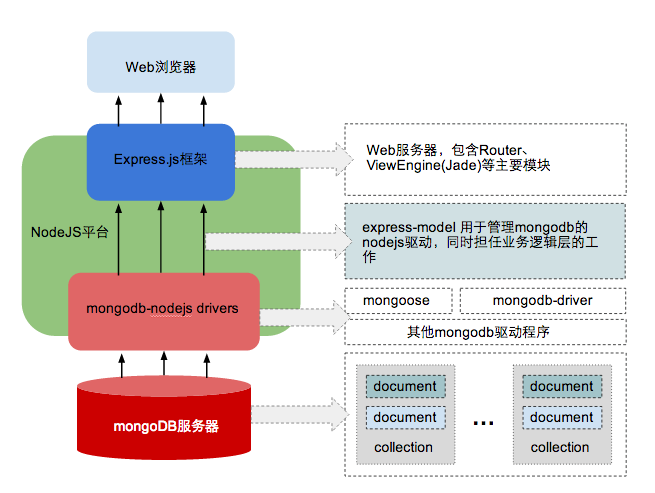
\includegraphics[width=1\textwidth]{./images/server-side-architecture.png}
  \caption{服务端架构图}
\end{figure}


\clearpage